% Shadow children on the coarse side of a 2D h-adaptive Cartesian mesh.
% The active refined cells form the same patch as in fig_dss_shadow.tex, while
% the gray overlays mark virtual children of coarse cells along its boundary.
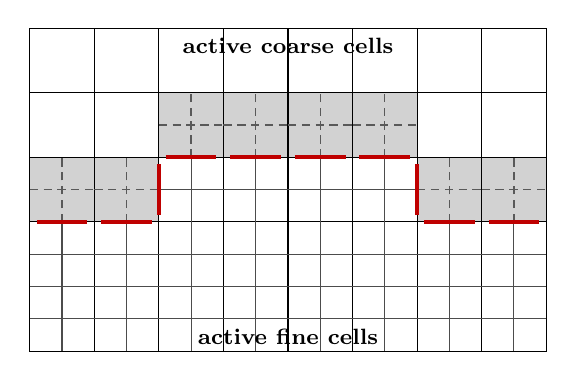
\begin{tikzpicture}[
                scale=0.82,
                coarse/.style={draw=black, thin},
                fine/.style={draw=black!70, line width=0.4pt},
                shadowfill/.style={fill=gray!35},
                shadow/.style={draw=black!65, densely dashed, line width=0.45pt},
                interface/.style={red!75!black, line width=1.45pt,
                    shorten >=2.5pt, shorten <=2.5pt},
                label/.style={font=\footnotesize\bfseries},
                legend/.style={font=\scriptsize, anchor=west}]
        % Active coarse cells whose virtual children cover the coarse side of the interface.
        \def\shadowparents{%
                0/2,1/2,6/2,7/2,%
                2/3,3/3,4/3,5/3}

        % Coarse background grid, including one intact layer above the shadow band.
        \draw[coarse] (0,0) rectangle (8,5);
        \foreach \i in {1,...,7} { \draw[coarse] (\i,0) -- (\i,5); }
        \foreach \j in {1,...,4} { \draw[coarse] (0,\j) -- (8,\j); }

        % Fine active cells: two globally refined layers and a raised central patch.
        \foreach \c in {0,...,7} {
                \draw[fine] (\c+0.5,0) -- (\c+0.5,2);
                \draw[fine] (\c,0.5) -- (\c+1,0.5);
                \draw[fine] (\c,1.5) -- (\c+1,1.5);
        }
        \draw[fine] (0,1) -- (8,1);
        \foreach \c in {2,...,5} {
                \draw[fine] (\c+0.5,2) -- (\c+0.5,3);
                \draw[fine] (\c,2.5) -- (\c+1,2.5);
        }

        % Overlay the virtual shadow children on coarse cells adjacent to the fine patch.
        \foreach \c/\r in \shadowparents {
                \fill[shadowfill] (\c,\r) rectangle (\c+1,\r+1);
                \draw[coarse] (\c,\r) rectangle (\c+1,\r+1);
                \draw[shadow] (\c+0.5,\r) -- (\c+0.5,\r+1);
                \draw[shadow] (\c,\r+0.5) -- (\c+1,\r+0.5);
        }

        % Original non-matching interface; its two halves become matching fine-shadow faces.
        \foreach \x in {0,1,6,7} { \draw[interface] (\x,2) -- (\x+1,2); }
        \foreach \x in {2,3,4,5} { \draw[interface] (\x,3) -- (\x+1,3); }
        \draw[interface] (2,2) -- (2,3);
        \draw[interface] (6,2) -- (6,3);

        % Labels and compact legend.
        \node[label] at (4,0.22) {active fine cells};
        \node[label] at (4,4.72) {active coarse cells};
\end{tikzpicture}
